% This is samplepaper.tex, a sample chapter demonstrating the
% LLNCS macro package for Springer Computer Science proceedings;
% Version 2.20 of 2017/10/04
%
\documentclass[runningheads]{llncs}
%
\usepackage{graphicx}
% Used for displaying a sample figure. If possible, figure files should
% be included in EPS format.
%
% If you use the hyperref package, please uncomment the following line
% to display URLs in blue roman font according to Springer's eBook style:
% \renewcommand\UrlFont{\color{blue}\rmfamily}
\usepackage{amsmath}

\begin{document}
%
\title{Deep triplet network adopting the kernel and the range space learning for Wi-Fi signature verification}
%
%\titlerunning{Abbreviated paper title}
% If the paper title is too long for the running head, you can set
% an abbreviated paper title here
%
\author{YoungWoong KWON\inst{1} \and
Jooyoung Kim \inst{1} \and
Kar-Ann Toh\inst{1}}
%
\authorrunning{F. Author et al.}
% First names are abbreviated in the running head.
% If there are more than two authors, 'et al.' is used.
%
\institute{Yonsei University \and
\email{lncs@springer.com}\\
\url{http://www.springer.com/gp/computer-science/lncs} \and
ABC Institute, Rupert-Karls-University Heidelberg, Heidelberg, Germany\\
\email{\{abc,lncs\}@uni-heidelberg.de}}
%
\maketitle              % typeset the header of the contribution
%
\begin{abstract}
The abstract should briefly summarize the contents of the paper in
15--250 words.

\keywords{First keyword  \and Second keyword \and Another keyword.}
\end{abstract}
%
%
%
\section{Introduction}

\subsection{Motivation}
i. Pros of In-Air WIFI CSI signature system
1) Cheap: Use commercial device
2) Easy: No additional devices is needed
3) Secure: Hard to forgery
ii. Cons of In-Air WIFI CSI signature system
1) Setting direction problem
a) Different direction -> Different feature is needed
b) Hard to set exactly same direction as authentication before
Size of signature can varies

\subsection{Contribution}
- Overcome cons of WIFI signature system
- Robust to signal direction, size

\section{Related Works}

\subsection{WIFI CSI}
- An In-Air Signature Verification System Using Wi-Fi Signals 

% Meaning of CSI
%[From Halperin paper]
CSI captures signal strength and phase information for OFDM subcarriers and between each pair of transmit-receive antennas.
It runs on a commodity 802.11n NIC, and records Channel State Information (CSI) based on the 802.11 standard.
The CSI contains information about the channel between sender and receiver at the level of individual data subcarriers, for each pair of transmit and receive antennas.
%[From Halperin End]

% Structure of CSI
%[From HC's ELM paper]
In a frequency domain, the CSI of sub-carrier $\mathbf{c}$ between transmitter(Tx) and receiver(Rx) can be modeled as 
$\mathnormal{R}_{c} = \mathbf{H}_{c}\mathnormal{T}_{c} +\mathnormal{N}$ where the $\mathnormal{R}_{c}$ and $\mathnormal{T}_{c}$  denote the received and the transmitted signal vector of dimension $\mathnormal{r}$ and $\mathnormal{t}$, respectively. The $\mathnormal{N}$ is the additive channel noise and $\mathbf{H}_{c}$ is the $\mathnormal{r}\times\mathnormal{t}$ channel matrix. The CSI of sub-carrier $\mathnormal{c}$ can be modeled as follows:
\begin{equation}
    \mathnormal{h}_{c} = \mid\mathnormal{h}_{c}\mid\mathnormal{e}^{\angle\theta},
\end{equation}
where $\mid\mathnormal{h}_{c}\mid$ and $\theta$ represent the amplitude and the phase of the sub-carrier, respectively.
%[From HC's ELM end]

\subsection{the kernel and the range space learning}

Multilayer feedforward neural networks has been widely used to feature extractor and classifier.
For traning the feedforward multilayer networks, non-gradient learning method by using linear matrix equation has invented recently. \cite{wang2018review}

This model avoids the problems of the deep learning model such as vanishing gradient and local minima. And except for the number of layers and number of neurons in the network, no more parameters are needed for the network configuration.

More recently, a new learning framework has been developed to train the weights of the deep networks by a series of kernel and range space projection method \cite{toh2018learning,toh2018gradient}.
This method allows to quickly learn the weights of the deep network with little system resources.
we adopted this method to mining negative samples for the training dataset.

%% Methods
\section{Proposed System}

In this section, we propose a direction-free identify verification system based on the Wi-Fi based in-air handwritten signature (will be called Wi-Fi signature signals hereafter). An overview of the proposed system utilizing the ConvNet \cite{lecun1998gradient} and the kernel and the range space projection learning (KAR space learning) \cite{toh2018learning,toh2018gradient} is shown in Fig.1.
Essentially, the Wi-Fi signature signals are preprocessed to create the input data for our network. Subsequently, the training dataset is moved to KAR space learning. KAR space learning generates triplet data by mining the hard positve and hard negative samples for given anchor signal.
generated triplet data flows into ConvNet structure. ConvNet extracts feature vectors by using filters.
ConvNet training is achived by triplet loss, which is formulated by the L-2 distance of feature vectors for the triplet. 
The following subsections detail the proposed method.

% Figure 1
\begin{figure}
    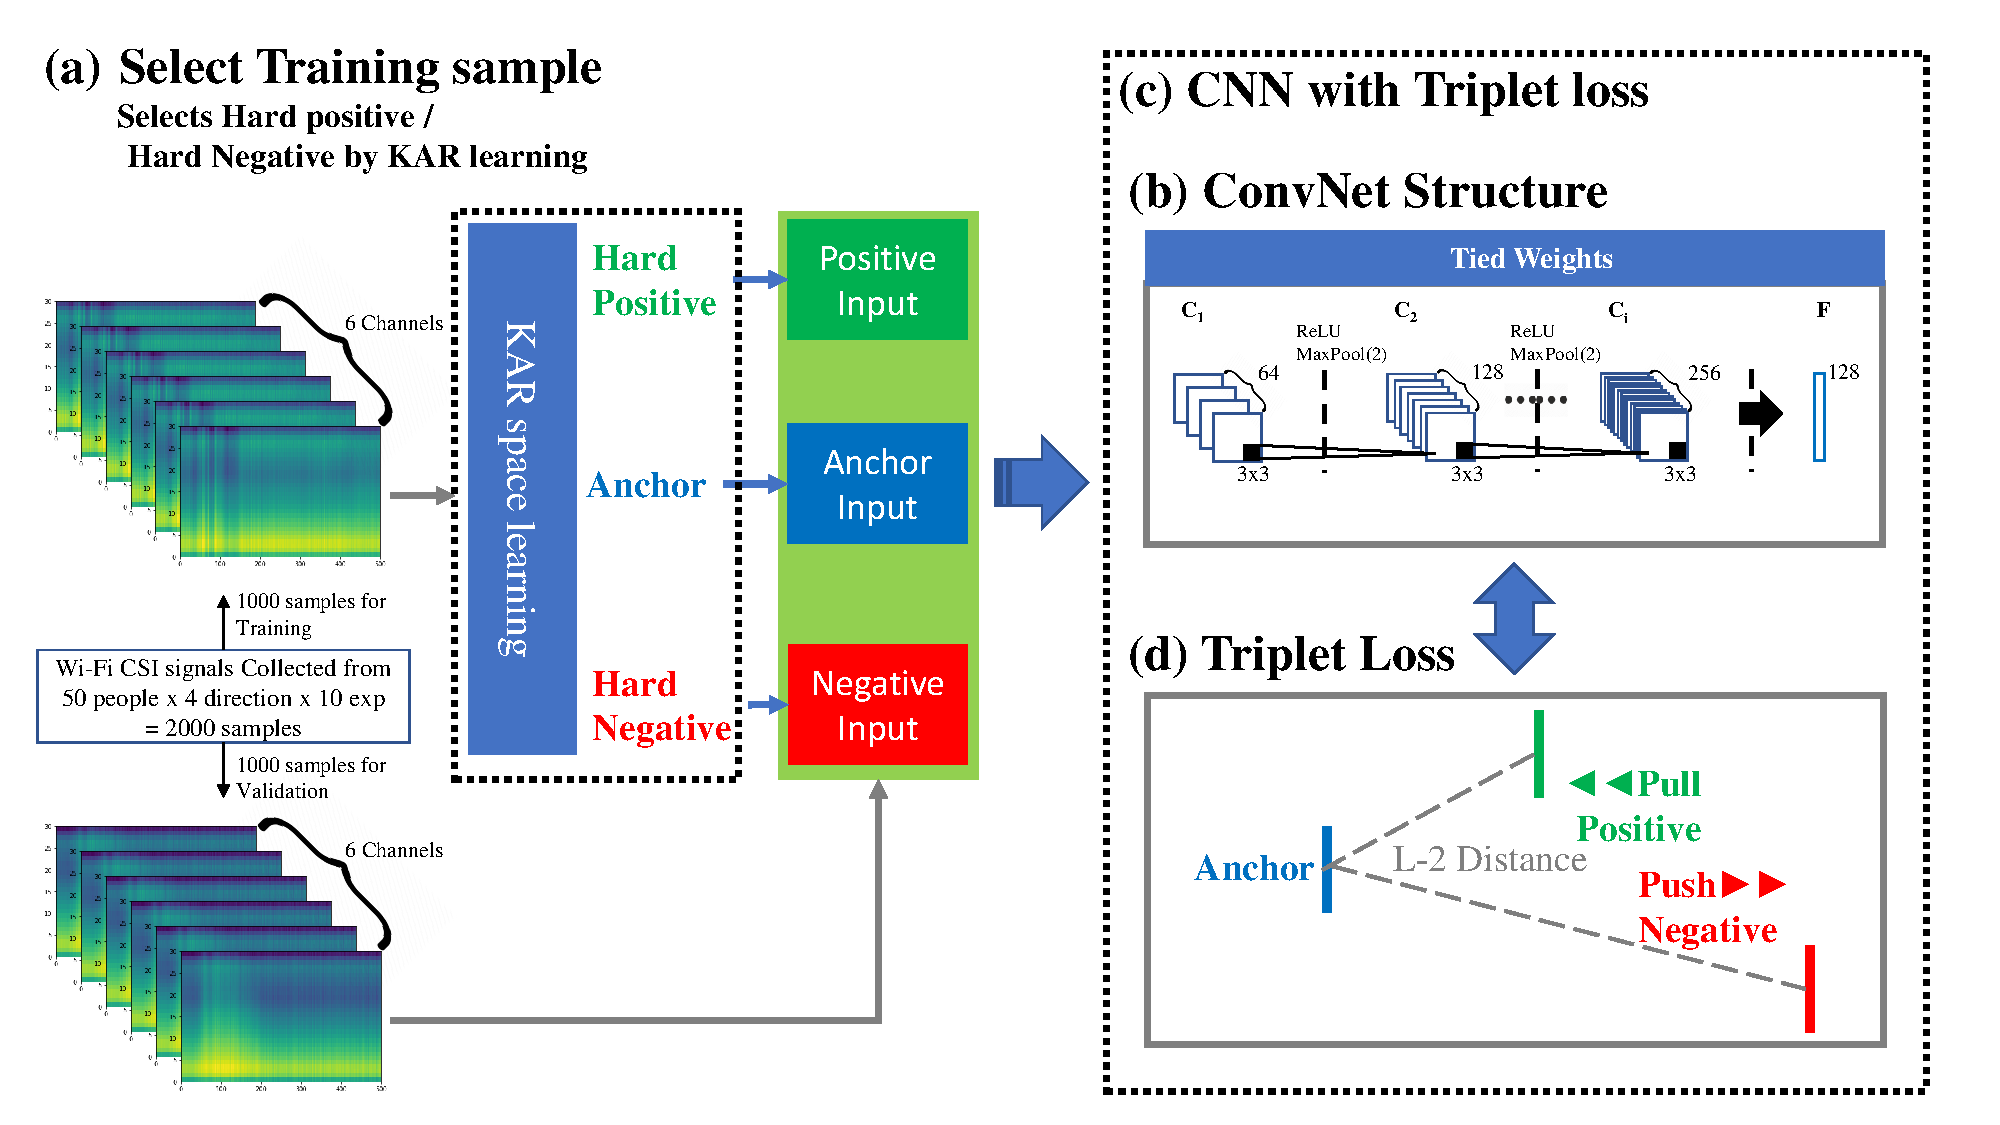
\includegraphics[width=\textwidth]{fig1_network_structure.pdf}
    \caption{Structure of the network} \label{fig1}
\end{figure}


% Methods: Triplet loss
\subsection{Triplet loss}

Our proposed networks utilizes the L-2 distance to calculate the triplet loss for given triplet input. For the $i_{th}$ anchor input signal $\mathbf{I}_{i,anc}$, triplet input can be generated by grouping positive input signal $\mathbf{I}_{i,pos}$ and negative input signal $\mathbf{I}_{i,neg}$.
positive input is drawn from the same identity for anchor signal and negative input is chosen from another identity for the anchor.
Generated triplet $\left\{\mathbf{I}_{i,anc},\mathbf{I}_{i,pos},\mathbf{I}_{i,neg}\right\}$ is the input to the ConvNet structure.
Let $\mathbf{x}_{i,anc}\in{\mathrm{R}}^{d\times1}$, $\mathbf{x}_{i,pos}\in{\mathrm{R}}^{d\times1}$ and $\mathbf{x}_{i,neg}\in{\mathrm{R}}^{d\times1}$ be three feature vectors extracted from the ConvNet structure. The triplet loss for the inputs can be calculated as follows:
\begin{equation}
loss = \sum_i^N { \left[ {\left\| {{\mathbf{x}_{i,anc}} - {\mathbf{x}_{i,pos}}} \right\|_2^2} -
{\left\| {{\mathbf{x}_{i,anc}} - {\mathbf{x}_{i,neg}}} \right\|_2^2}  + \alpha \right]_+},
\end{equation} 
where $\alpha$ is the margin between distances from anchor to positive and anchor to negative, N is size of the mini-batch. (+) means greater number between zero or calculated loss.

% Methods: KAR learning

\subsection{Triplet mining by the kernel and the range space learning}

% importance of selecting hard pos/neg
Regarding to \cite{schroff2015facenet}, it is important to take hard positive and hard negative sample for faster convergence of the loss when training triplet networks.
hard positive sample means distance between feature vectors from positive signal to anchor signal is the greatest, while hard negative sample means distance between feature vectors from negative signal to anchor signal is the smallest.

% methods of KAR learning
since we don't know which is the hard sample before training the network, we train multilayer feedforward neural network to mine the hard positive and the hard negative from traning dataset.
For training multilayer neural network, we adopted gradient-free the kernel and the range (KAR) space projection learning. \cite{toh2018learning,toh2018gradient}.

% Karnet structure and mining samples.
Let the training dataset $\mathbf{X}\in{\mathrm{R}}^{m \times (n+1)}$ and $\mathbf{G}\in{\mathrm{R}}^{m \times n}$ is network outputs.
Multilayer neural network structure is shown below:

\begin{equation}
    \mathbf{G} = \sigma\left(\left[\mathbf{1},\sigma\left(\dots\left[\mathbf{1},\sigma\left(\left[\mathbf{1},\sigma\left(\mathbf{X}\mathbf{W}_{1}\right)\right]\mathbf{W}_{2}\right)\right]\dots\mathbf{W}_{(i-1)}\right)\right]\mathbf{W}_{i}\right),
\end{equation}

$\mathbf{W}_{1}\in{\mathrm{R}}^{(n+1) \times h_{1}}$,$\mathbf{W}_{2}\in{\mathrm{R}}^{(h_{1}+1) \times h_{2}}$,$\dots,\mathbf{W}_{i}\in{\mathrm{R}}^{(h_{(i-1)}+1) \times n}$,$\mathbf{1}=\left[1,\dots,1\right]^{T}\\
\in{\mathrm{R}}^{m \times 1}$ and $\sigma(.)$ is activation function.

when all weights have been learned, for given anker signal, hard negative samples can be mined among the distance of network output of desired signal $\mathbf{G}$ is below the threshold.

% training KARnet
Network learning is archived using one-hot encoded target $\mathbf{Y}\in{\mathrm{R}}^{m \times n}$ instead of network output $\mathbf{G}$.
After that, we have the weight matrix $\mathbf{W}_{1}\dots\mathbf{W}_{i}$ to train. the weight matrix can be separated into weights and bias term as
$\mathbf{W}_{2}\dots\mathbf{W}_{i}$ = 
$\begin{bmatrix}
\mathbf{w}_{2}^{T}\\\mathnormal{W}_{2}
\end{bmatrix}
\dots
\begin{bmatrix}
\mathbf{w}_{i}^{T}\\\mathnormal{W}_{i}
\end{bmatrix}$.

after assign random weights to $\mathbf{W}_{1}\dots\mathbf{W}_{i}$ , we get $\mathbf{W}_{1}$. it is solved as follows:

\begin{equation}
    \left[\sigma^{-1}\left(\mathbf{Y}\right)-\mathbf{1}\cdot\mathbf{w}_{i}^{T}\right]\mathnormal{W}_{i}^\dagger = 
    \sigma\left(\dots\left[\mathbf{1},\sigma\left(\left[\mathbf{1},\sigma\left(\mathbf{X}\mathbf{W}_{1}\right)\right]\mathbf{W}_{2}\right)\right]\dots\mathbf{W}_{(i-1)}\right)
\end{equation}

%\begin{multline*}
\begin{equation}
    \begin{aligned}
        \Rightarrow
        \biggl[\sigma^{-1}\biggl(
        \dots
        \biggl[\sigma^{-1}\biggl(
            \left[\sigma^{-1}\left(\mathbf{Y}\right)-\mathbf{1}\cdot\mathbf{w}_{i}^{T}\right]\mathnormal{W}_{i}^\dagger
        \biggr)
        - \mathbf{1}\cdot\mathbf{w}_{(i-1)}^{T}\biggr]\mathnormal{W}_{(i-1)}^{\dagger}
        \dots\biggr)\\
        - \mathbf{1}\cdot\mathbf{w}_{2}^{T}\biggr]\mathnormal{W}_{2}^{\dagger} 
        = \sigma\left(\mathbf{X}\mathbf{W}_{1}\right)
    \end{aligned}
\end{equation}
%\end{multline*}

%\begin{multline*}
\begin{equation}
    \begin{aligned}
        \Rightarrow
        \mathbf{X}^{\dagger}\sigma^{-1}\biggl(
        \biggl[\sigma^{-1}\biggl(
        \dots
        \biggl[\sigma^{-1}\biggl(
            \left[\sigma^{-1}\left(\mathbf{Y}\right)-\mathbf{1}\cdot\mathbf{w}_{i}^{T}\right]\mathnormal{W}_{i}^\dagger
        \biggr)
        - \mathbf{1}\cdot\mathbf{w}_{(i-1)}^{T}\biggr]\mathnormal{W}_{(i-1)}^{\dagger}
        \dots\biggr)\\
        - \mathbf{1}\cdot\mathbf{w}_{2}^{T}\biggr]\mathnormal{W}_{2}^{\dagger}
        = \mathbf{W}_{1}
    \end{aligned}
\end{equation}
%\end{multline*}

after getting $\mathbf{W}_{1}$, $\mathbf{W}_{2}$ can also be optimized

%\begin{multline*}
\begin{equation}
    \begin{aligned}
        \Rightarrow
        \left(\sigma\left(\mathbf{X}\mathbf{W}_{1}\right)\right)^{\dagger}
        \biggl(\dots
        \biggl[\sigma^{-1}\biggl(
            \left[\sigma^{-1}\left(\mathbf{Y}\right)-\mathbf{1}\cdot\mathbf{w}_{i}^{T}\right]\mathnormal{W}_{i}^\dagger
        \biggr)
        - \mathbf{1}\cdot\mathbf{w}_{(i-1)}^{T}\biggr]\mathnormal{W}_{(i-1)}^{\dagger}
        \dots\biggr)\\
        = \mathbf{W}_{2}
    \end{aligned}
\end{equation}
%\end{multline*}

Repeat this process recursively until all weight maxtrix values are obtained.
finally, $\mathbf{W}_{i}$ can be obtained as follows:

\begin{equation}
    \mathbf{W}_{i} = \left[\mathbf{1},\sigma\left(\dots\left[\mathbf{1},\sigma\left(\left[\mathbf{1},\sigma\left(\mathbf{X}\mathbf{W}_{1}\right)\right]\mathbf{W}_{2}\right)\right]\dots\mathbf{W}_{(i-1)}\right)\right]^{\dagger}\sigma^{-1}\left(\mathbf{Y}\right),
\end{equation}


% Methods: ConvNets
\subsection{ConvNet Structures}

To design the proposed networks, we firstly need to select the feature extracting networks which convert the triplet data into a feature vector. In this work, we utilize the ConvNet structure \cite{lecun1998gradient} as a feature extractor since the three-dimensional data format of our preprocessed input signal can be regarded as an image data format with multiple channels. 

Our ConvNet structure (See Fig~\ref{fig1} (b)) for the network consists of $i$ convolutional layers $\mathbf{C}_{i}$ and one fully-connected layer $\mathbf{F}$. The number of convolutional filters to be trained in each layer is empirically chosen as $\{64, 128, ...,  2^{6+i}\}$, with fixed filter size of $3\times3$ and stride of 1. The Rectified Linear (ReLU) function as an activation function and the max-pooling layers are applied between each convolutional layers. The features from the last convolutional layer are directly flattened into a single vector.
we used sigmoid activation at ConvNet output and L-2 normalize output vectors to prevent negative distance when calculating triplet loss.

%Since the networks utilize three ConvNet structures which ties the weights each other, noting here that three structures described in Fig~\ref{fig1} (b) are actually the same model.

\section{Experiments}

% Dataset
\subsubsection{Dataset}
 To evaluate validation performance of proposed system, Wi-Fi CSI signature dataset from \cite{moon2017air} was used.
 % pre-processing
 Since every Wi-Fi signature signal has different data size, we firstly adopted the gradient operation with respect to the time instance to measure the short time energy. Data points with the highest short-time energy within the time period are then manually selected as the starting and the ending points of the in-air signature action. Subsequently, the Fast Fourier Transform based re-sampling method \cite{moon2017air} is implemented to unify the length of the signals. As a result, three-dimensional Wi-Fi signature signals with unified data size are obtained as the input of the ConvNet structure in the network.
 % description
 we utilized 2000 Wi-Fi CSI signature signals (4 directions $\times$ 50 identities $\times$ 10 samples) which is dimension of (500 packets $\times$ 30 subcarriers $\times$ 6 antennas). 
 
% network shape

% network parameters

% Network Learning
\subsubsection{ConvNet structure}
 We impose a triplet loss objective on our classifier.
This objective is combined with standard backpropagation algorithm.
 We initialized all network weights in the convolutional layers from a normal distribution with zero-mean and a standard deviation of 0.01. Biases were also initialized from a normal distribution, but with mean 0.5 and standard deviation 0.01.
 all layers are L-2 regularized using parameters of 0.0002. for output layer, regularization is 0.001

 For KARnet trainied multilayer neural networks, we set 2 layer and number of neurons are [1024,128]. initialized as uniform distribution over [0, 1).
 activation and inverse activation functions are [arctan, tan].


\section{Conclusion}

%
% ---- Bibliography ----
%
% BibTeX users should specify bibliography style 'splncs04'.
% References will then be sorted and formatted in the correct style.
%
%\bibliographystyle{splncs04}
%\bibliography{mybibliography}
%


%\begin{thebibliography}{8}

\bibliographystyle{splncs04}
\bibliography{bib_acpr}

%\end{thebibliography}

\end{document}